\documentclass{emulateapj}

\newcommand\be{\begin{equation}}
\newcommand\ee{\end{equation}}

\title{Newton and Maxwell}
\date{}


\begin{document}

\maketitle

% Begin discussion of Newton’s laws of motion 
\section{Newton’s Laws} 
Newton’s first law says: ‘‘Every body continues in its state of rest, 
or of uniform motion in a right line, unless it is compelled to change 
that state by forces impressed upon it."

Newton’s second law is 
\be
\vec F = m \vec a \label{Newton2}
\ee
where $\vec F$ is the force on a particle of mass m, 
and $\vec a$ is the particle’s acceleration.

Newton's third law says that for every action, there is an equal and opposite reaction.

\begin{center}
\begin{figure}[h]
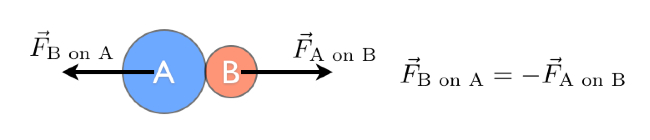
\includegraphics[scale = 0.35]{n3l.png}
\caption{Newton's third law.}
\end{figure}
\end{center}

Wrapping up, Newton's second law (\ref{Newton2}) allows us to predict the future.

% Begin discussion of Maxwell’s equations 
\section{Maxwell’s Equations} 
Maxwell’s equations include Gauss’s law, which reads 
\be
\oint \vec E \cdot d\vec a = \frac{Q}{\epsilon_0} 
\ee
in integral form.\newline
Faraday law:
\be
\oint \vec E \cdot d\vec s = -\frac{d\Phi}{dt} 
\ee
Amp\'ere law:
\be
\vec \nabla \times \vec B = \mu_0 \vec J + \mu_0 \epsilon_0 \frac{\partial \vec E}{\partial t} 
\ee
And finally, $\vec \nabla \cdot \vec B = 0$


\end{document}